\documentclass[12pt,a4paper,onecolumn]{article}
\usepackage[utf8]{inputenc}
\usepackage[T1]{fontenc}
\usepackage[french]{babel}

% ------------------------- Color table ----------------------------------------

\usepackage{siunitx}
\usepackage{booktabs}
\usepackage{multirow}
\usepackage[table]{xcolor}
\definecolor{maroon}{cmyk}{0,0.87,0.68,0.32}
% ------------------------------------------------------------------------------

\usepackage{amscd}
\usepackage{amsthm}
\usepackage{physics}
\usepackage[left=2.2cm,right=2.2cm,top=2cm,bottom=2cm]{geometry}
\usepackage{textcomp,gensymb} %pour le °C, et textcomp pour éviter les warning
\usepackage{graphicx} %pour les images
\usepackage{caption}
\usepackage{subcaption}
\usepackage[colorlinks=true,
	breaklinks=true,
	citecolor=blue,
	linkcolor=blue,
	urlcolor=blue]{hyperref} % pour insérer des liens
\usepackage{epstopdf} %converting to PDF
\usepackage[export]{adjustbox} %for large figures

\usepackage{array}
\usepackage{dsfont}% indicatrice : \mathds{1}


% -------------------------- Mathematics ---------------------------------------
\graphicspath{{images/}} % For the images path
% ------------------------------------------------------------------------------

% -------------------------- Mathematics ---------------------------------------
\usepackage{mathrsfs, amsmath, amsfonts, amssymb}
\usepackage{bm}
\usepackage{mathtools}
\usepackage[Symbol]{upgreek} % For pi \uppi different from /pi
\newcommand{\R}{\mathbb{R}} % For Real space


% -------------------------- Footers / header ----------------------------------
\usepackage{fancyhdr}
\pagestyle{fancy}
% ------------------------------------------------------------------------------


% -------------------------- Code format ---------------------------------------
\usepackage[numbered,framed]{matlab-prettifier}
\lstset{
	style              = Matlab-editor,
	basicstyle         = \mlttfamily,
	escapechar         = '',
	mlshowsectionrules = true,
}
% ------------------------------------------------------------------------------

% ------------------------- Blbiographie --------------------------------------
\usepackage[backend=biber, style=ieee]{biblatex}
\usepackage{csquotes} %for biblatex warning
\addbibresource{biblio.bib}
% ------------------------------------------------------------------------------

%\setcounter{tocdepth}{4} %Count paragraph
%\setcounter{secnumdepth}{4} %Count paragraph
\usepackage{float}

\usepackage{graphicx} % for graphicspath

\usepackage{array,tabularx}
\newcolumntype{L}[1]{>{\raggedright\let\newline\\\arraybackslash\hspace{0pt}}m{#1}}
\newcolumntype{C}[1]{>{\centering\let\newline\\\arraybackslash\hspace{0pt}}m{#1}}
\newcolumntype{R}[1]{>{\raggedleft\let\newline\\\arraybackslash\hspace{0pt}}m{#1}}


% ------------------------ General informations --------------------------------
\title{Unsupervised learning: from big data to low-dimensional representations}
\author{Vincent MATTHYS, Pirashanth RATNAMOGAN, Othmane SAYEM}
\date{}
\graphicspath{{images/}{../images/}} % For the images path
\lhead{Face Clustering and Motion Segmentation Challenge}
\chead{}
\rhead{}
\lfoot{}
\cfoot{\thepage}
\rfoot{}
% ------------------------------------------------------------------------------

% ---------------------------- Mofidy {sub}section size -----------------------
\usepackage{sectsty}
\sectionfont{\fontsize{12}{15}\selectfont}
\subsectionfont{\fontsize{12}{15}\selectfont}
% ------------------------------------------------------------------------------


\begin{document}
\thispagestyle{empty}

\maketitle

\begin{center}
	\rule[11pt]{5cm}{0.5pt}

	\textbf{\LARGE \textsc{Project 2}\\Face Clustering\\and Motion Segmentation Challenge}
	\vspace{0.5cm}

	Vincent MATTHYS\\Pirashanth RATNAMOGAN\\Othmane SAYEM\\

	\{vincent.matthys, pirashanth.ratnamogan, othmane.sayem\}@ens-paris-saclay.fr

	\rule{5cm}{0.5pt}

	\vspace{1.5cm}
\end{center}

\begin{tabularx}{0.9\textwidth}{@{} l X r @{} }
	{\textsc{Master MVA}}     &  & \textsc{Unsupervised learning} \\
	\textsc{ENS Paris Saclay} &  & {Instructor: René VIDAL}       \\
\end{tabularx}

% \tableofcontents

\clearpage
\thispagestyle{fancy}

\setcounter{section}{-1}
\section{This project is to be done in MATLAB or Python and in groups of three students.  Please report
  which student did which part. Each student should also email me a grade (0-100\%=best) for the work of his/her mates.}

We did the projet in Python. We have tried to share the work fairly. Hence during the first phase of the project, Vincent focused in the implementation of the Spectral Clustering and in the Clustering error while Pirashanth worked in the  Sparse Subspace Clustering with noisy data implementation and Othmane worked in the K-Subspaces algorithm implementation.
Because we have faced lot of troubles during the implementation we helped each other in view of successfully produce operational implementations of the three algorithms.
After this first part made essentially of implementations and debugging, Othmane and Pirashanth dealed essentially with the Face clustering (question 2) and Vincent worked on Motion Segmentation (question 3).

\section{Clustering Algorithms. Implement the Spectral Clustering (SC) algorithm (Algorithm 4.5), K-Subspaces algorithm (Algorithm 6.1) and Sparse Subspace Clustering (SSC) algorithm with noisy data (Algorithm 8.5 and 8.6). You can use the MATLAB kmeans function (or python) inside SC.}
\label{section_algos}

We have implemented the three algorithms and an implementation of the "best" precision rate using the hungarian algorithm implemented within the function. \\
We also tried to improve the outcome that we obtained in the face clustering challenge, by using the methods described in the book "Generalized Principal Component Analysis". Indeed, we tried to use a preprocessing using PCA when applying the K-subspaces algorithm (that allows to cut the computation time) and we try to use SSC with sparse outlying data (we doesn't succeed to make it converge properly).

\section{Face clustering}

\subsection{Report the clustering error for individuals 1-2 for different choices of the parameters \(\sigma\) and \(K\) for SC (when constructing a Gaussian affinity with K-NN), number of restarts for K-subspaces, and \(\lambda\) for SSC.}

Here we report the clustering errors for individuals 1-2 for different choice of the parameters in the three algorithms that we have implemented.

\begin{table}[H]
	\centering
	\begin{tabular}{l|r|r}
		\toprule
		{}    k & sigma  & error rate      \\
		\midrule
		10      & 100    & 49\%            \\
		10      & 500    & 49\%            \\
		10      & 1000   & 49\%            \\
		10      & 10000  & 49\%            \\
		10      & 100000 & 50 \%           \\
		5       & 50     & 49\%            \\
		5       & 100    & \textbf{37.5\%} \\
		5       & 500    & 49\%            \\
		5       & 1000   & 49\%            \\
		3       & 100    & 43.75\%         \\
		3       & 500    & 46\%            \\
		3       & 1000   & 48.43\%         \\
		1       & 100    & 49\%            \\
		1       & 500    & 48\%            \\
		1       & 1000   & 48 \%           \\
		\bottomrule
	\end{tabular}
	\caption{Clustering precision for individuals 1-2 using Spectral Clustering}
\end{table}

\begin{table}[H]
	\centering
	\begin{tabular}{l|r|r}
		\toprule
		{}    d & replicates & error rate     \\
		\midrule
		3       & 1          & 48.4\%         \\
		3       & 2          & 6.2\%          \\
		3       & 3          & \textbf{5.4\%} \\
		2       & 3          & 25.8\%         \\
		4       & 3          & 49.2\%         \\
		5       & 3          & 50\%           \\
		6       & 3          & 49.2\%         \\
		10      & 3          & 46.8\%         \\
		\bottomrule
	\end{tabular}
	\caption{Clustering precision for individuals 1-2 using K-Subspaces}
\end{table}

\begin{table}[H]
	\centering
	\begin{tabular}{l|r|r}
		\toprule
		{}    \(\tau\) & \(\mu_2\) & error rate               \\
		\midrule

		\(1   \)       & 500       & 46\%                     \\
		\(0.2 \)       & 500       & 45\%                     \\
		\(10^{-4}\)    & 20        & 33.5\%                   \\
		\(10^{-4}\)    & 30        & 33.5\%                   \\
		\(10^{-4}\)    & 40        & 33.6\%                   \\
		\(10^{-4}\)    & 50        & 33.6\%                   \\
		\(10^{-5}\)    & 20        & 10.1\%                   \\
		\(10^{-5}\)    & 30        & \textbf{8.5\%}           \\
		\(10^{-5}\)    & 40        & 8.5\%                    \\
		\(10^{-5}\)    & 50        & 8.5\%                    \\
		\(10^{-5}\)    & 1000      & 8.6\%                    \\
		\(10^{-6}\)    & ....      & $D^{1/2}$ not invertible \\
		\bottomrule
	\end{tabular}
	\caption{Clustering precision for individuals 1-2 using SSC}
\end{table}

As we can see parameters choice have an important role in the algorithms performance.
To set smartly the parameters we can use some basic rule of thumbs:
\begin{enumerate}
	\item For the SC one can set the parameter $\sigma$ using the intra-cluster standard deviation
	\item For the K-Subsaces, the higher the number of replicates is, the better the final outcome will be. However because each restart are costly we will never exceed a number of 3 restarts. As described in class images of the same face under varying illumination lie near an approximately nine-dimensional linear subspace. However we get better outcome by setting this linear subspace very low. Indeed it allows to find a more discriminative model.
	      The big dimension of each vector (D) makes the algorithm costly in terms of computation time, one alternative would be to reduce the dimension using PCA, by taking only d principal components (depends on the dimension of clusters)  and applying the algorithm to the resulting data matrix.

	\item For the SSC algorithm, using \textbf{Lemma 8.28} we set the $\tau$ as a multiple of the calculated $\tau_{\text{min}}$. For the parameter $\mu_2$, we used a large choice of values then deduced an interval of values that assures the best performance.
\end{enumerate}

The Tables 1,2 and 3 allow to have an overview of how our three algorithms could perform in the face clustering take. \\
Spectral Clustering is performing really poorly in the face clustering task. That could be explain, by the fact that to compute the affinity matrix we are using K-NN based on the euclidean distance. This distance isn't the more adequate for this kind of high dimensional data. \\
K-subspaces and SSC are performing well in some cases but the error rate is really sensitive to how we set the parameters.

Because all the tests that we did are really time consuming, we couldn't do the same type of test for each subset of individuals 1-10, and 1-20, 1-30, 1-38. Hence, as suggested we will set the parameters for the remaining tests that we have to compute. We will take the parameters that better performs in the part with the individuals 1-2.

\subsection{Once you have chosen the best parameters for each method, report the clustering errors for individuals 1-2, 1-10, and 1-20, 1-30, 1-38, and analyze the clustering error as a function of the number of groups.}

Here we report the clustering errors for individuals 1-2, 1-10, and 1-20, 1-30, 1-38. In those computations, the parameters are set by using the parameters that performs best in the clustering for individuals 1-2.

\begin{table}[H]
	\centering
	\begin{tabular}{l|r|r}
		\toprule
		{}    nb of individuals & error rate \\
		\midrule
		1-2                     & 37.5\%     \\
		1-10                    & 80\%       \\
		1-20                    & 86\%       \\
		1-30                    & 89\%       \\
		1-38                    & 88\%       \\
		\bottomrule
	\end{tabular}
	\caption{Clustering precision for various number of individuals using SC}
\end{table}

\begin{table}[H]
	\centering
	\begin{tabular}{l|r|r}
		\toprule
		{}    nb of individuals & error rate \\
		\midrule
		1-2                     & 5.4\%      \\
		1-10                    & 64\%       \\
		1-20                    & 70\%       \\
		1-30                    & 72\%       \\
		1-38                    & 75\%       \\
		\bottomrule
	\end{tabular}
	\caption{Clustering precision for various number of individuals using K-subspaces}
\end{table}


\begin{table}[h]
	\centering
	\begin{tabular}{l|r|r}
		\toprule
		{}    nb of individuals & error rate \\
		\midrule
		1-2                     & 8.5\%      \\
		1-10                    & 56\%       \\
		1-20                    & 65\%       \\
		1-30                    & 67\%       \\
		1-38                    & -          \\
		\bottomrule
	\end{tabular}
	\caption{Clustering precision for various number of individuals using SSC}
\end{table}

\begin{figure}[H]
	\centering
	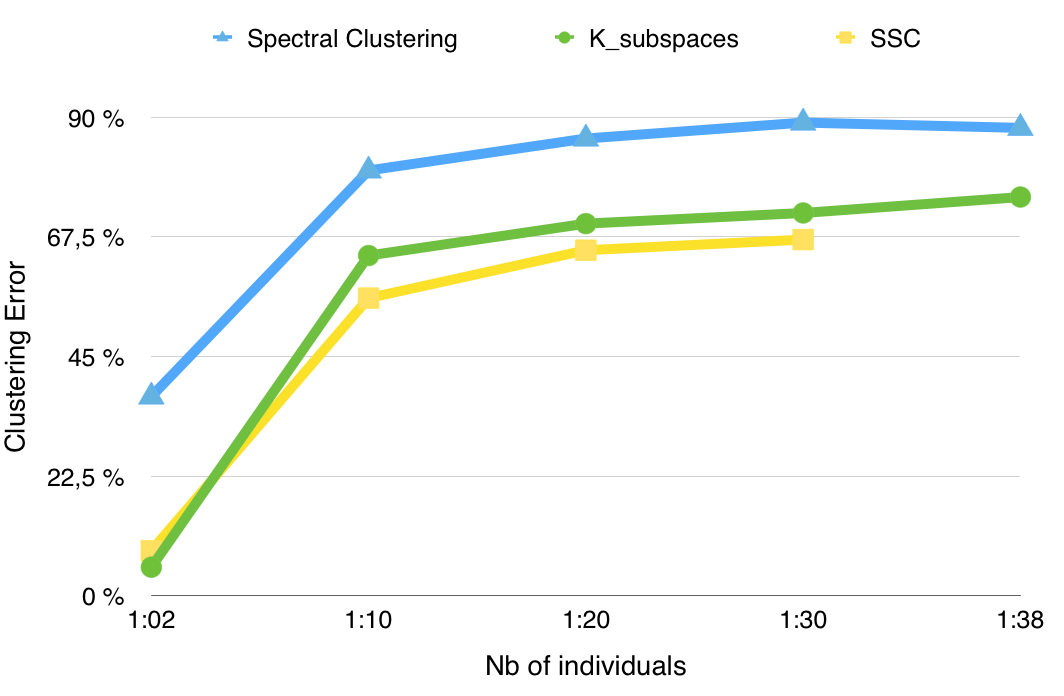
\includegraphics[width = 0.9\textwidth]{nb_individuals.png}
	\caption{Clustering error for each method, applied to various numbers of compared individuals}
	\label{fig_1}
\end{figure}

As we can see in the Table 4,5,6 the performance of the three algorithms are not quite good. Yet, Figure~\ref{fig_1} for the chosen parameters, we notice that for all numbers of individuals, SSC gets the best results compared to the two other methods. Unsupervised face clustering is a really complex task. One can remember the following plots presented by R.Vidal:

\begin{figure}[H]
	\centering
	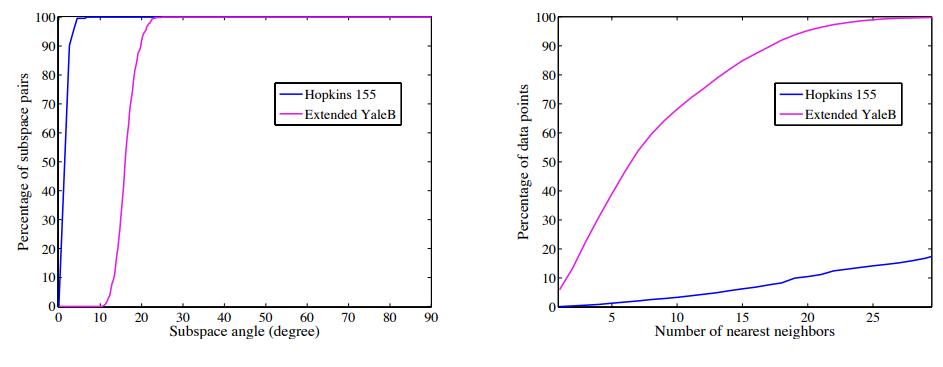
\includegraphics[width = 0.9\textwidth]{Challenge-face-clustering.PNG}
	\caption{Challenge face clustering, from R.Vidal \cite{vidal2016PCA} page}
	\label{fig_challenge_face_clustering}
\end{figure}


We have two difficulties in the clustering task in Extended YaleB database: angles between subspaces are small, Nearby points are in different subspaces.


These difficulties make that it will be almost impossible for the SC and the K-subspaces algorithms to perform well because they are based on these points. Hence, before running the tests, we could only hope the SSC with noising data algorithm to perform well. K-subspaces, perform well with individuals 1-2 but its performance decreases when increasing the number of individuals. SSC also performs badly even if it produces the best outcome, as shown in the Figure1. As suggested in the book, another possibility is to use the SSC with sparse outlying entries that seems to perform well in the face clustering task.


\section{Motion Segmentation}

By applying the algorithms in section~\ref{section_algos} to the feature point trajectories from the Hopkins155 dataset, we aim to quantify the results obtained. The clustering error for different choices of the parameters \(\sigma\) and K for SC (when constructing a Gaussian affinity with K-NN), number of restarts for K-subspaces, and \(\lambda\) for SSC are compared next.

The figure~\ref{fig_challenge_face_clustering} shows the difference in terms of neighborhood between the face clustering problem and the movie segmentation problem. One can expects the parameters and the results to be different in both cases. The percentage of sequences for which the clustering error is below a given value is represented to quantify the results obtained by qualitatively looking at the area under this curve. In order to perform the clustering part, the algorithms were given the true number of clusters, available in the Hopkins155 dataset as the maximum of the label in each \textit{ground\_truth.mat}.

\subsection{Spectral clustering}

For the spectral clustering, the influence of \(K\) in the computation of the affinity matrix is presented in figure~\ref{fig_motion_sc_res_k}. The area under the curve is larger with K, except for the case \(K=1\), but the effect decrease with \(K\). Moreover, two different behaviours can be observed: \(K \leq 3\) and \(K \geq 4\) where a substantial early gap in term of misclassification appears. To conclude, as long as the complexity allows it, a bigger choice of \(K\) has to be preferred.

\begin{figure}[H]
	\centering
	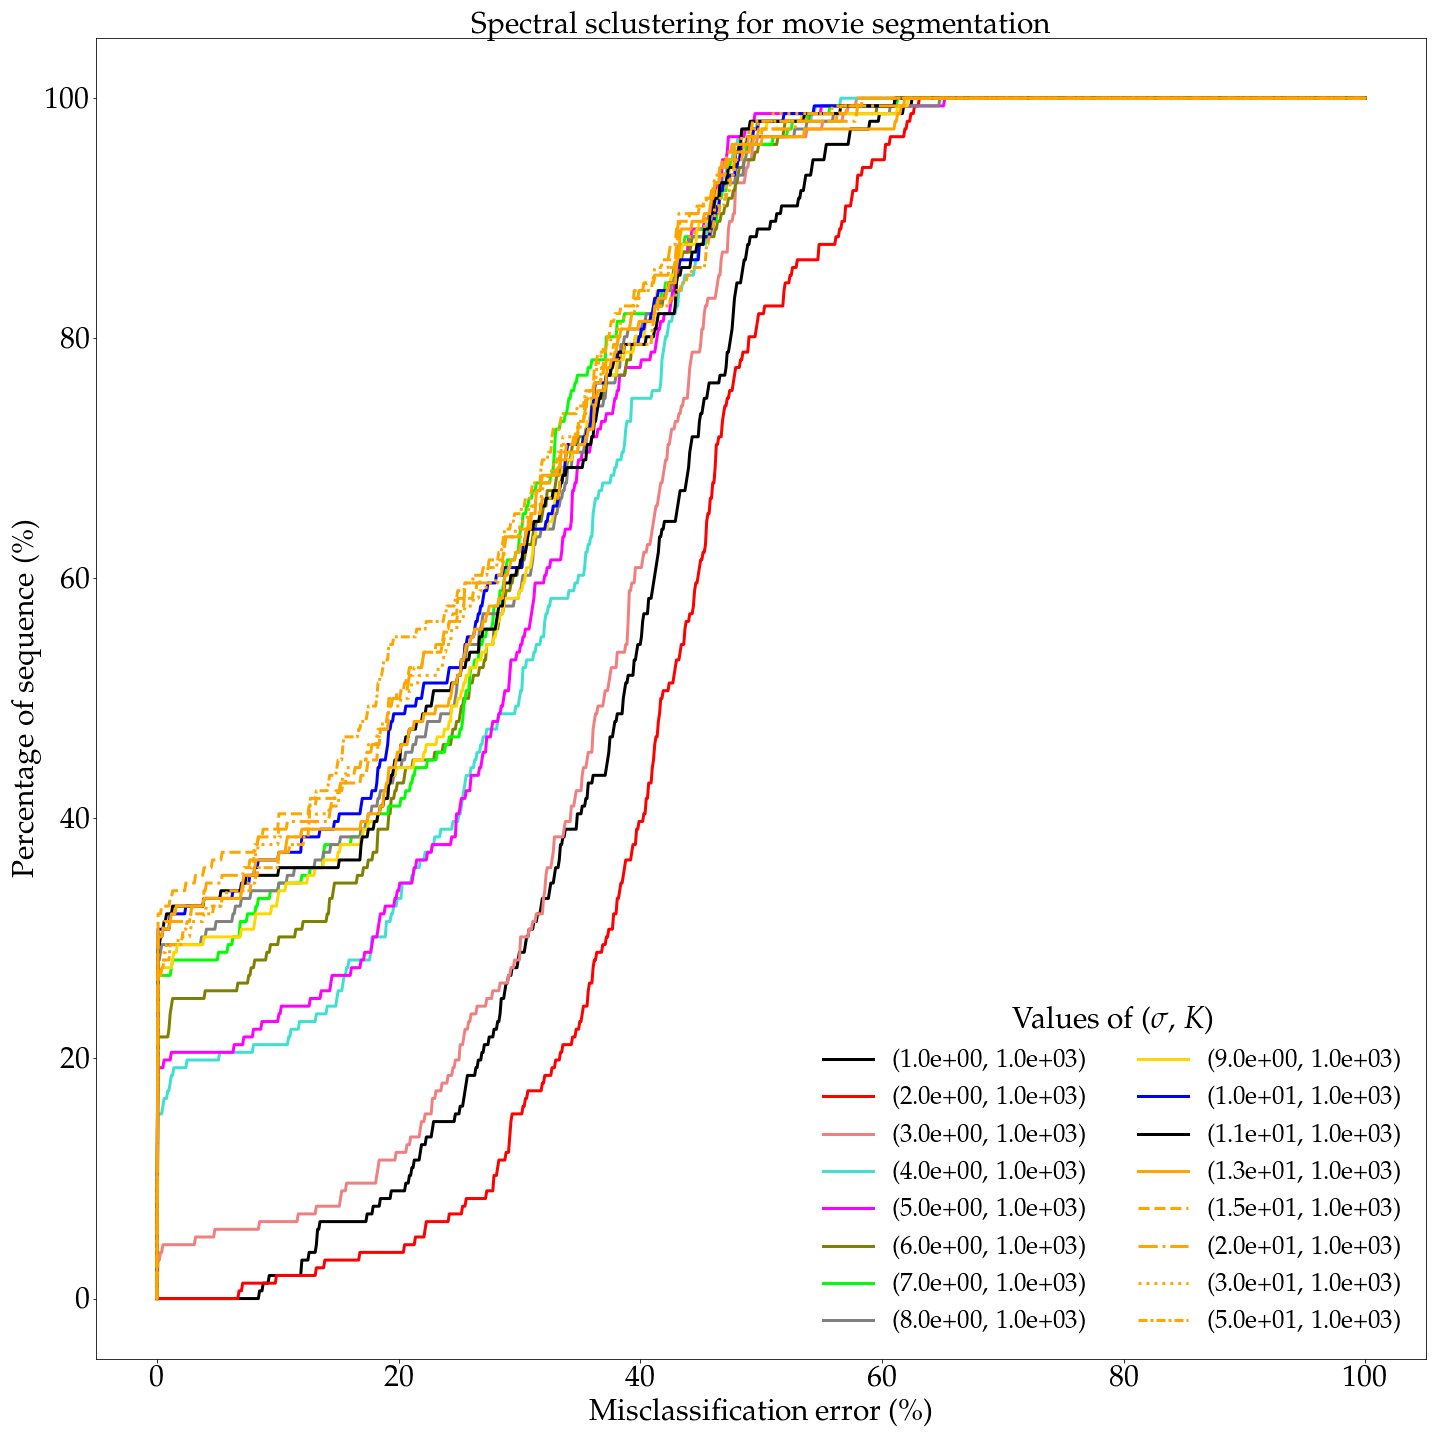
\includegraphics[width = 0.9\textwidth]{SC_1e3}
	\caption{Case of spectral clustering, with different parameters \(K\) for the computation of the affinity matrix. The percentage of sequences for which the clustering error is less than or equal to a given percentage of error is represented in different colors corresponding to a given value of \(K\)}
	\label{fig_motion_sc_res_k}
\end{figure}

The influence of \(\sigma\) is studied in figure~\ref{fig_motion_sc_res_sigma}. Here, two different values of \(K\) are represented for \(\sigma \in \{10^i\}_{i = 0..5}\). There is no noticeable behaviour here, and we can approximately say that the major parameter is \(K\).

\begin{figure}[H]
	\centering
	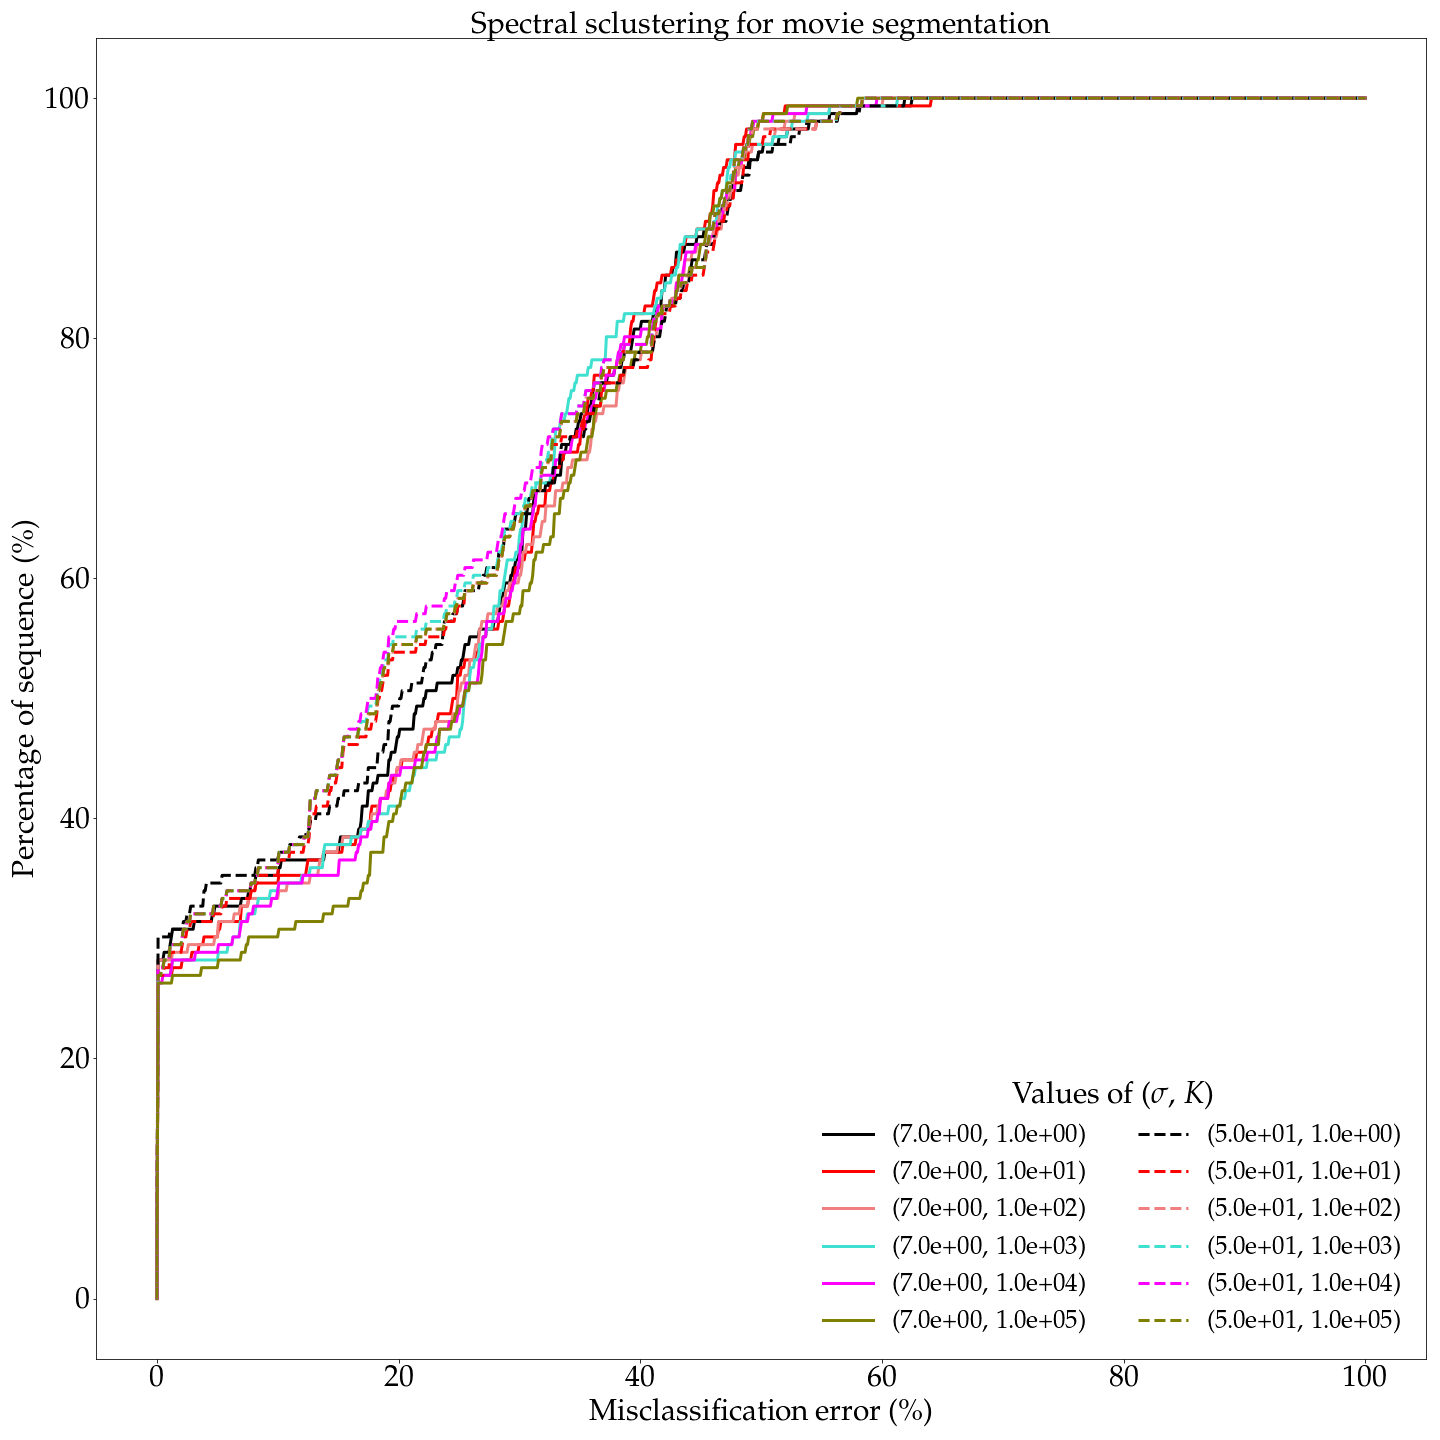
\includegraphics[width = 0.9\textwidth]{SC_k_7_50}
	\caption{Case of spectral clustering, with different parameters \(\sigma\) for the computation of the affinity matrix. The percentage of sequences for which the clustering error is less than or equal to a given percentage of error is represented in different colors corresponding to a given value of \(\sigma\). Two values of \(K\), 7 and 50 are represented.}
	\label{fig_motion_sc_res_sigma}
\end{figure}

\subsection{Ksubspaces}

When applying Ksubspaces to movie segmentation, the dimensions of the target clusters have to be known. We therefore can look at the singular values of the matrix of feature point trajectories, as proposed by R.Vidal in \cite{vidal2016PCA}¸ to get a good approximation with 4 dimensional subspace for every motion. In case of movie segmentation the influence of the number of restarts is observed in figure~\ref{fig_motion_ksub_res}. The single restart profile differs from the other, due to the randomness of the initialization in that case which is not counterbalanced by the number of restarts. The larger the number of restarts, the larger the area under the curve : it couldn't have been another way. To conclude, a largest number of restarts has to be preferred, to smooth the initial states and to get higher probabilities to get the global maximum.

\begin{figure}[H]
	\centering
	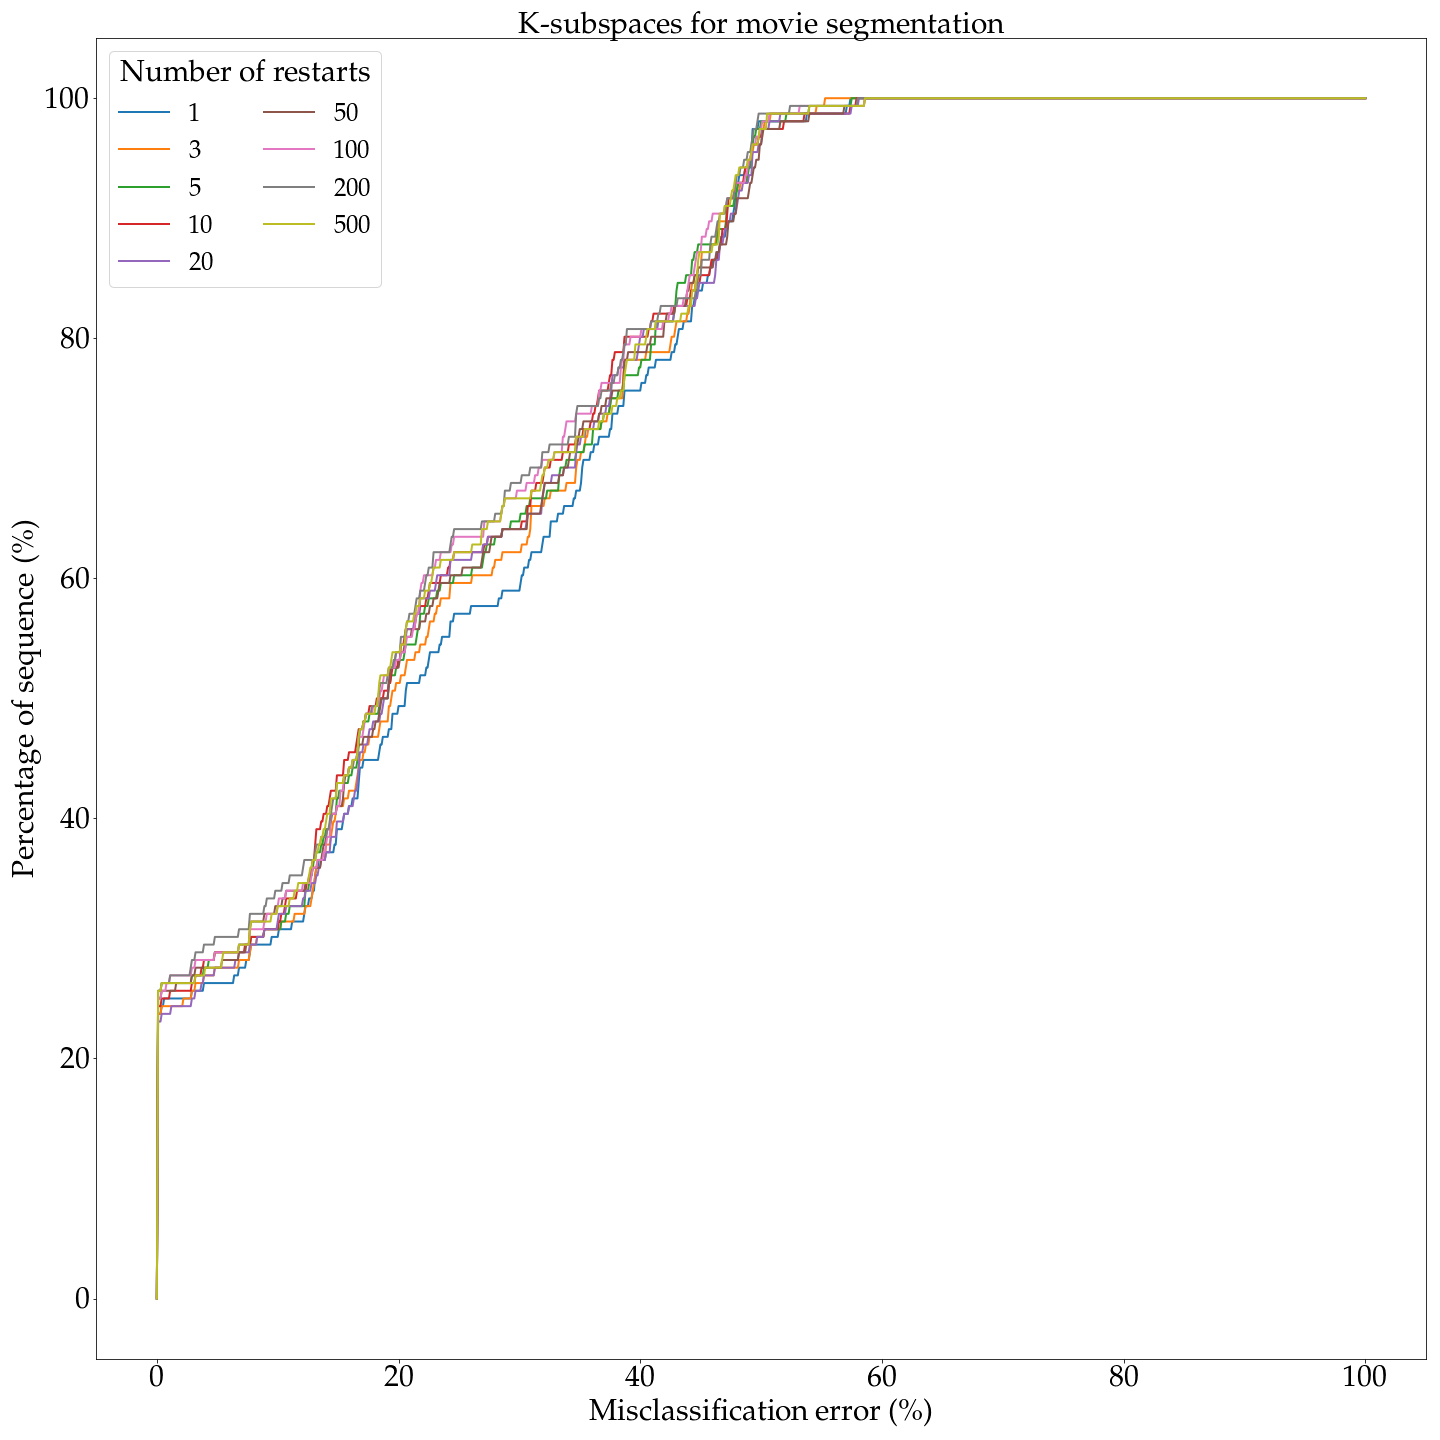
\includegraphics[width = 0.9\textwidth]{k_sub}
	\caption{Case of k-subspaces, with different number of restarts. The percentage of sequences for which the clustering error is less than or equal to a given percentage of error is represented in different colors corresponding to a given number of restarts.}
	\label{fig_motion_ksub_res}
\end{figure}


\subsection{Sparse spectral clustering}
The influence of \(\tau\) parameter for sparse spectral clustering applying to movie segmentation with the Hopkins155 data-set is observed in figure~\ref{fig_motion_SSC_tau_res}. The larger area under the curve is obtained for \(\tau = 10^4\) which is very different for the values obtained in the face clustering problem, with \(10^9\) order of magnitude.


\begin{figure}[H]
	\centering
	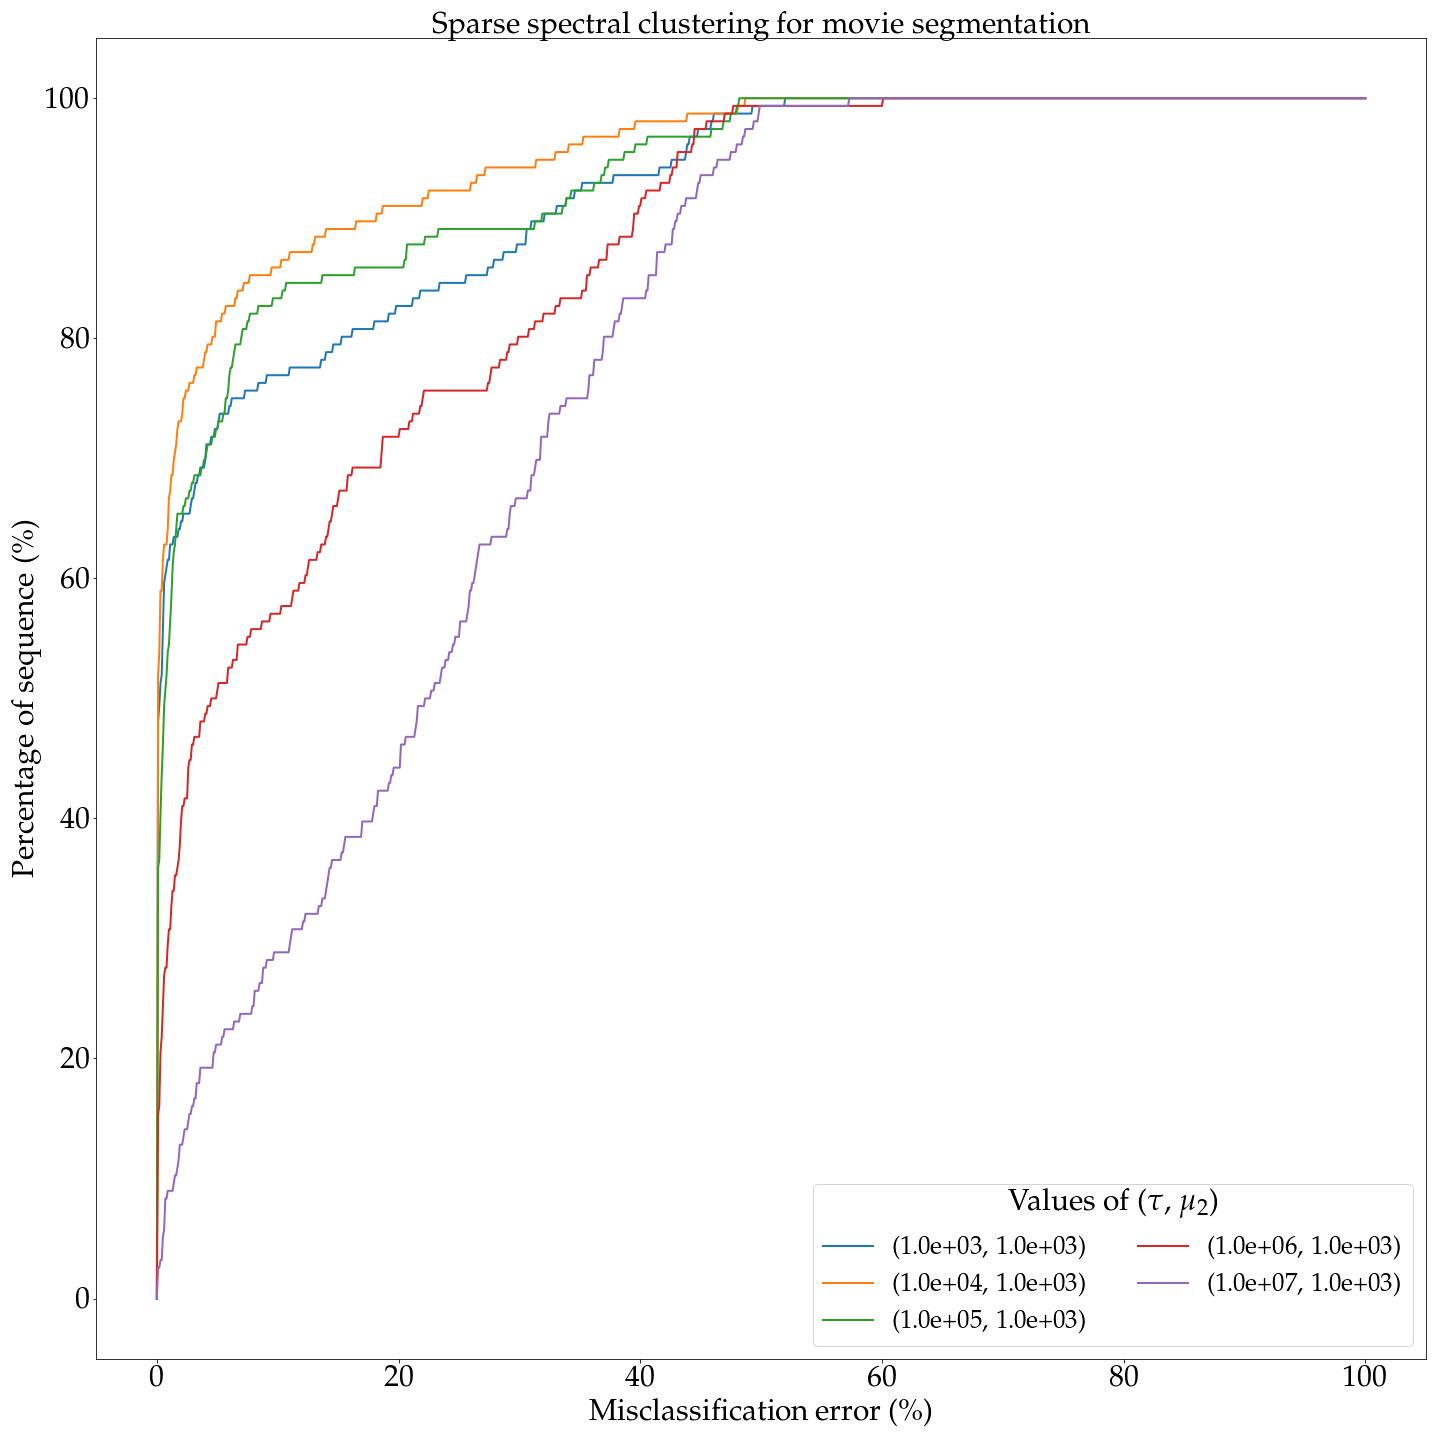
\includegraphics[width = 0.9\textwidth]{SSC_tau}
	\caption{Case of sparse spectral clustering for \(\mu_2 = 10^3\) and for different values of \(\tau\). The percentage of sequences for which the clustering error is less than or equal to a given percentage of error is represented in different colors corresponding to a given \(\tau\).}
	\label{fig_motion_SSC_tau_res}
\end{figure}

For this specific value of \(\tau\) we looked for the best \(\mu_2\) parameter. The results obtained are visible in figure~\ref{fig_motion_SSC_mu2_res}. We can clearly distinguish the profile obtaining the higher area under the curve, for \(\mu_2 = 10^{4}\). It leads to our conclusion, that optimal parameters for SSC applied to movie segmentation, based on this dataset, is \(\tau = 10^4, \mu_2 = 10^{4}\).

\begin{figure}[H]
	\centering
	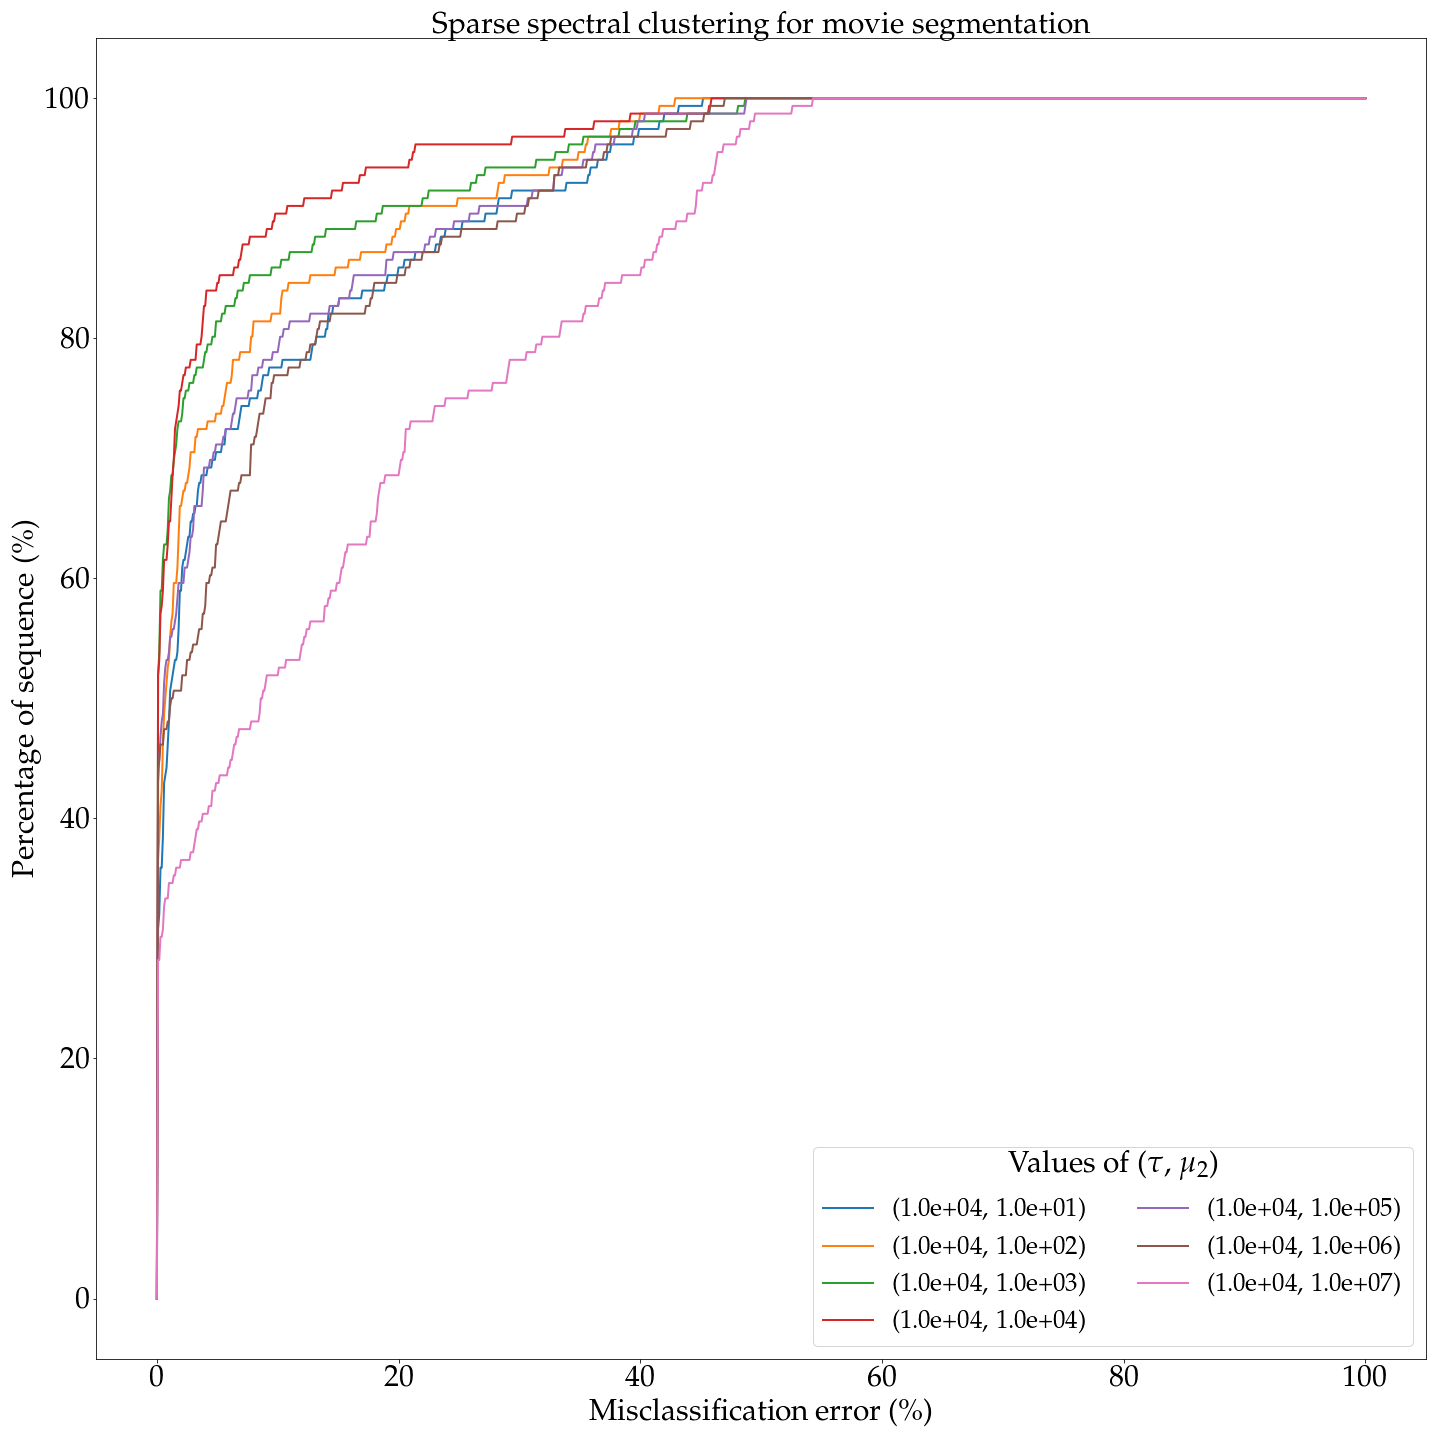
\includegraphics[width = 0.9\textwidth]{SSC_mu2}
	\caption{Case of sparse spectral clustering for \(\tau = 10^4\) and for different values of \(\mu_2\). The percentage of sequences for which the clustering error is less than or equal to a given percentage of error is represented in different colors corresponding to a given \(\mu_2\).}
	\label{fig_motion_SSC_mu2_res}
\end{figure}


\subsection{Comparison}

Finally, the best parameters for the three algorithms are chosen, and the resulting curves are presented in figure~\ref{fig_motion_auc_compare_res}. It's clear that the only algorithm presenting \(AUC >> 0.5\) is the SSC one. In fact, as we have seen in figures~\ref{fig_motion_SSC_tau_res},~\ref{fig_motion_SSC_mu2_res}, the only algorithm with such an \(AUC\) is SSC, supposing that the spatial data structure is not convenient for the two others clustering algorithms. In fact, if SSC is working, it does mean that the subspaces are independants, or disjoints, and that the dimension of the subspaces are very closed. On the other hand, as the local distance, on which is based spectral clustering fails to capture structure nearby closed subspaces, we could expect the poor results obtained by this algorithm, as the subspace angles, shown in figure~\ref{fig_1} in Hopkins155 data-set are really small in comparison with the Extended YaleB dataset.

\begin{figure}
	\centering
	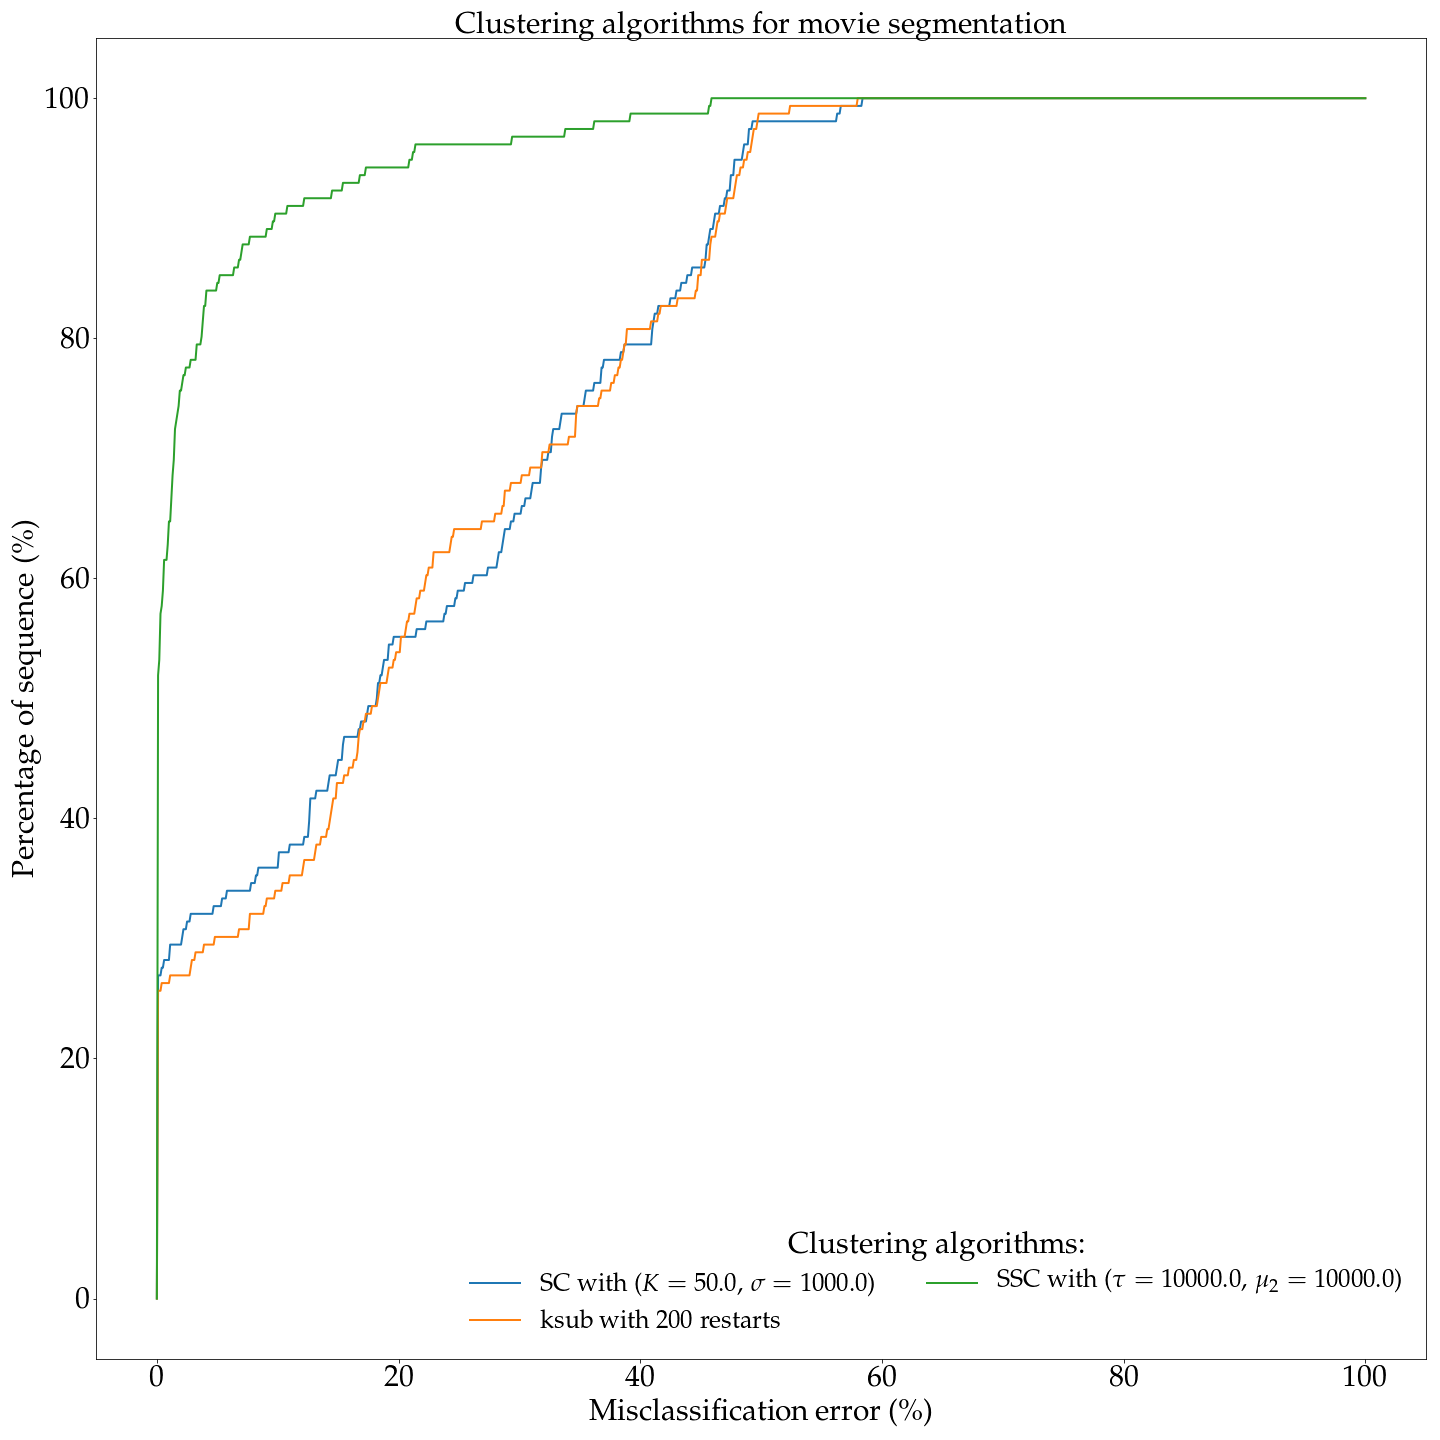
\includegraphics[width = 0.9\textwidth]{auc_compare}
	\caption{Applications to movie segmentation with the best parameters for three clustering algorithms. The percentage of sequences for which the clustering error is less than or equal to a given percentage of error.}
	\label{fig_motion_auc_compare_res}
\end{figure}


\printbibliography

\end{document}
